\documentclass[11pt]{article}
\usepackage[UTF8]{ctex}
\usepackage[a4paper]{geometry}
\geometry{left=2.0cm,right=2.0cm,top=2.5cm,bottom=2.5cm}

\usepackage{comment}
\usepackage{booktabs}
\usepackage{graphicx}
\usepackage{diagbox}
\usepackage{amsmath,amsfonts,graphicx,amssymb,bm,amsthm}
%\usepackage{algorithm,algorithmicx}
\usepackage[ruled]{algorithm2e}
\usepackage[noend]{algpseudocode}
\usepackage{fancyhdr}
\usepackage{tikz}
\usepackage{graphicx}
\usetikzlibrary{arrows,automata}
\usepackage{hyperref}
\usepackage{float}
\usepackage{tikz}
\usepackage{tikz-qtree}

\setlength{\headheight}{14pt}
\setlength{\parindent}{0 in}
\setlength{\parskip}{0.5 em}

\newtheorem{theorem}{Theorem}
\newtheorem{lemma}[theorem]{Lemma}
\newtheorem{proposition}[theorem]{Proposition}
\newtheorem{claim}[theorem]{Claim}
\newtheorem{corollary}[theorem]{Corollary}
\newtheorem{definition}[theorem]{Definition}
\newtheorem*{definition*}{Definition}

\newenvironment{problem}[2][Problem]{\begin{trivlist}
		\item[\hskip \labelsep {\bfseries #1}\hskip \labelsep {\bfseries #2.}]}{\hfill$\blacktriangleleft$\end{trivlist}}
\newenvironment{answer}[1][Answer]{\begin{trivlist}
		\item[\hskip \labelsep {\bfseries #1.}\hskip \labelsep]}{\hfill$\lhd$\end{trivlist}}

\begin{document}
	\pagestyle{fancy}
	\lhead{Peking University}
	\chead{}
	\rhead{Introduction to the Theory of Computation, 2024 Spring}
	\begin{center}
		{\LARGE \bf Homework 2}\\
		{Due: 2024-4-11 23:59 \quad$|$\quad 7 Problems, 100 Pts}
		{Name: 胡宇阳, ID: 2200013065}
	\end{center}
	\begin{problem}{1.(12 points)}
		Give context-free grammars that generate the following languages. In all parts the alphabet $\Sigma$ is $\{0, 1\}$.
		
		(1) $\{w \mid w \text{ starts and ends with the same symbol}\}$.
		
		(2) $\{w \mid w \text{ is a palindrome}\}$.
	\end{problem}
	\begin{answer}
		(1) CFL $C=(V,\Sigma,R,S)$, 满足 $V=\{A,B\},\Sigma=\{0,1\},S=\{A\}$,
		
		$R:A\rightarrow 0\mid 1\mid 0B0\mid 1B1,B\rightarrow \varepsilon\mid0B\mid1B$
		
		(2) CFL $C=(V,\Sigma,R,S)$, 满足 $V=\{A\},\Sigma=\{0,1\},S=\{A\}$,
		
		$R:A\rightarrow \varepsilon\mid0\mid 1\mid 0A0\mid 1A1$
	\end{answer}
	\begin{problem}{2.(12 points)}
		For any language $A$ with alphabet $\Sigma$, let 
		\begin{align*}
			\text{PREFIX}(A) = \{w \mid wv \in A \text{ for some } v \in \Sigma^*\}
		\end{align*}
		Show that the class of context-free languages is closed under the PREFIX operation.
	\end{problem}
	\begin{answer}
		\textcircled{1} 对于 CFL $A=(V,\Sigma,R,S)$, $V=\{v_1,v_2,\cdots,v_n\},\Sigma=\{c_1,c_2,\cdots,c_m\}$
		
		建立新的 CFL $B=(V^\prime,\Sigma^\prime,R^\prime,S^\prime)$, 满足 $V^\prime=\{v_1,v_2,\cdots,v_n\}\cup\{v_1^\prime,v_2^\prime,\cdots,v_n^\prime\},\Sigma^\prime=\Sigma,S^\prime=S$ (也就是将变元复制了一份)
		
		对于 $str=u_1u_2\cdots u_n$, 定义 $P(str)=u_1^\prime u_2^\prime\cdots u_n^\prime$ 表示 $\forall i\in\{1,2,\cdots,n\}, u_i=v_j\vee u_i=v_j^\prime\Rightarrow u_i^\prime=v_j^\prime,u_i\in V\Rightarrow u_i^\prime=u_i$ (相当于把所有变元加一个 $\prime$)
		
		同时记 $NP(str)$ 为 $P^{-1}(str)$ (相当于把所有变元去掉一个 $\prime$)
		
		$R^\prime$ 是满足 \begin{itemize}
			\item $\forall (v_i\rightarrow str=u_1u_2\cdots u_t)\in R, (v_i^\prime\rightarrow P(str))\in R^\prime$
			
			\item $\forall (v_i\rightarrow str=u_1u_2\cdots u_t)\in R,\forall j\in\{0,1,2,\cdots,t\}, (v_i\rightarrow P(u_1u_2\cdots u_{j-1})u_j)\in R^\prime$  
		\end{itemize}
		的最小的集合.
		
		对于 $r=(v_i^\prime\rightarrow P(str))\vee(v_i\rightarrow P(u_1u_2\cdots u_{j-1})u_j)\in R^\prime$, 记 $ORI(r)=(v_i\rightarrow str=u_1u_2\cdots u_t)\in R$, 也就是 $R^\prime$ 从 $R$ 中哪个元素生成的.
		
		\textcircled{2} 下证 $B\subseteq\text{PREFIX}(A)$:
		
		对于 $B$ 中生成的字符串 $str=x_1x_2\cdots x_p$,
		
		存在一个生成规则的顺序 $r_1,r_2,\cdots,r_q\in R^\prime$, 记 $ORI(str)=ORI(r_1),ORI(r_2),\cdots,ORI(r_q)$ 为在同样位置按照原有规则替换生成的字符串.
		
		下使用数学归纳法证 $str$ 为 $ORI(str)$ 的前缀:
		
		归纳结论为: 由 $ORI(r_1),ORI(r_2),\cdots,ORI(r_k)$ 生成的字符串 $ORI(str_k)$, 由 $r_1,r_2,\cdots,r_k$ 生成的字符串 $str_k$, 满足 $NP(str_k)$ 为 $NP(ORI(str_k))$ 的前缀.
		
		在 $k=0$ 时, 均为初始状态, 结论显然成立.
		
		下假设 $k-1$ 时成立, 现对 $ORI(str_{k-1})$ 进行第 $k$ 次替换 $(v_i\rightarrow u_1u_2\cdots u_t)$, 
		
		若替换位置不在 $str_{k-1}$ 末尾, 由 $R^\prime$ 的性质 $2$, 非末尾元素的一定有 $\prime$, 所以在 $str_{k-1}$ 上进行的相应的替换为 $v_i^\prime\rightarrow P(u_1u_2\cdots u_t)$, 由于 $NP(u_1u_2\cdots u_t)=NP(P(u_1u_2\cdots u_t))$, $NP(str_k)$ 依然为 $NP(ORI(str_k))$ 的前缀.
		
		若替换位置在 $str_{k-1}$ 的末尾, 而 $NP(P(u_1u_2\cdots u_t))$ 和 $NP(P(u_1u_2\cdots u_{j-1})u_j)$ 是 $NP(u_1u_2\cdots u_t)$ 的前缀, 在最后替换后, $NP(str_k)$ 依然为 $NP(ORI(str_k))$ 的前缀.
		
		则归纳结论成立, 由于最后字符串不会有变元, 而 $ORI(str)\in A$所以 $B\subseteq \text{PREFIX}(A)$.
		
		\textcircled{3} 下证 $\text{PREFIX}(A)\subseteq B$:
		
		取 $A$ 中元素 $str=s_1s_2\cdots s_n$, 任取其前缀 $pstr=s_1s_2\cdots s_m\in\text{PREFIX}(A),(m\leq n)$.
		
		则 $str$ 存在一套替换规则 $r_1,r_2,\cdots,r_t\in R$, 对于每次替换 $r_i=(v_j\rightarrow u_{i,1}u_{i,2}\cdots u_{i,k_i})$, 每一个非变元与最终结果中的非变元 $pstr=s_1s_2\cdots s_m$ 进行一一映射, 将所有替换中对应 $s_{m+1},s_{m+2},\cdots,s_n$ 的非变元全部删除, 由替换的性质, 删除的必然为替换的后缀, $r_i^\prime=(v_j\rightarrow P(u_{i,p}u_{i,p+1}\cdots u_{i,q-1})u_{i,q})$ (将变元中除了末端的全部加上 $\prime$), 由 $R^\prime$ 定义, $r_i^\prime\in R^\prime$. 则存在 $r_1^\prime,r_2^\prime,\cdots,r_t^\prime\in R^\prime$, $r_1^\prime,r_2^\prime,\cdots,r_t^\prime$ 生成 $pstr$.
		
		所以 $\text{PREFIX}(A)\subseteq B$
	\end{answer}
	\begin{problem}{3.(12 points)}
		(1) Prove that the language $L = \{0^{2^n} \mid n \ge 0\}$ is not context free.
		
		(2) Let $B$ be the language of all palindromes over $\{0, 1\}$ containing an equal number of 0s and 1s. Show that $B$ is not context free.
	\end{problem}
	\begin{answer}
		(1) 若 $L$ 为 CFL, 则 $\exists p,\forall s\in L,|s|\geq p,s=uvxyz,uv^ixy^iz\in L\wedge |vy|>0\wedge|vxy|\leq p$.
		
		取 $s=0^{2^p}$, 则 $\exists k\in\{1,2,\cdots,2^p\}, 0^{2^p+nk}\in L$, 而 $0^{2^p+k}\in L\Rightarrow k=2^p\Rightarrow0^{2^p+2k}\notin L$
		
		所以 $L$ 不是 CFL.
		
		(2) 若 $L$ 为 CFL, 则 $\exists p,\forall s\in L,|s|\geq p,s=uvxyz,uv^ixy^iz\in L\wedge |vy|>0\wedge|vxy|\leq p$.
		
		取 $s=0^p1^{2p}0^p$, 若 $v,y$ 均只有 $0,1$, 则 $v=0^n,y=1^n$ 或者 $v=1^n,y=0^n$, 则 $uv^2xy^2z=0^{p+n}1^{2p+n}0^p$ 或者 $uv^2xy^2z=0^p1^{2p+n}0^{p+n}$, 不是回文序列.
		
		由于两个 $0$ 序列间隔有 $2p$, 而 $|vxy|\leq p$, 所以 $v,y$ 不可能同时有 $0,1$ 所以一个有一个没有. 不妨 $v=0^a1^b,y=1^{a+b}$, 则 $uv^2xy^2z=0^p1^b0^a1^{2p+a+b}0^p$ 不是回文序列.
		
		所以 $L$ 不是 CFL.
	\end{answer}
	\begin{problem}{4.(16 points)}
		Define a two-dimensional Turing machine to be a TM where each of its tapes is an infinite grid (and the read/write head can move not only Left and Right but also Up and Down). Show that for every $T: \mathbb{N} \rightarrow \mathbb{N}$ and every Boolean function $f$ , if $f$ can be computed in time $T(n)$ using a two-dimensional TM, then it can also be computed by a standard (one-dimensional) TM in time $O(T(n)^2)$. ($T$ may not be time constructible)
	\end{problem}
	\begin{answer}
		对于二维图灵机 $TM$, 构造函数 $f:(x,y)\rightarrow z$, 为二维到一维的映射, 
	
		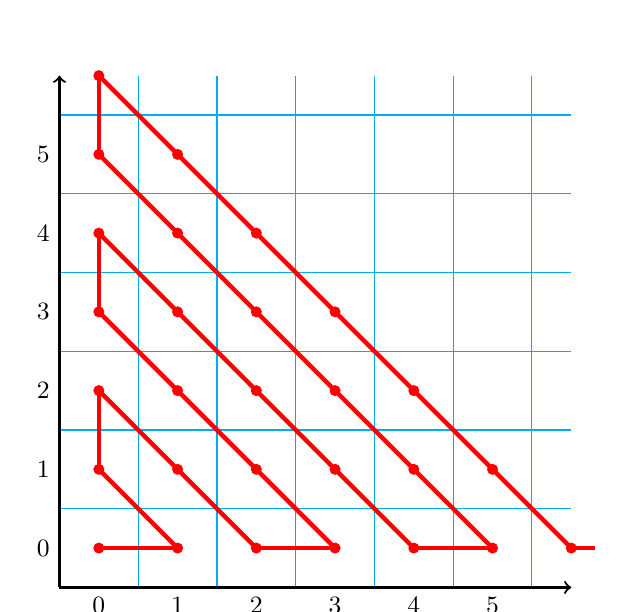
\begin{tikzpicture}
			\foreach \x in {0,1,2,3,4,5} {
				\node[below] at (\x+0.5,0) {\small\x};
			}
			\foreach \y in {0,1,2,3,4,5} {
				\node[left] at (0,\y+0.5) {\small\y};
			}
			\draw[step=1, cyan] (0,0) grid (6.5,6.5);
			\draw[->, thick, black] (0,0) -- (0,6.5) node[left] {$~$};
			\draw[->, thick, black] (0,0) -- (6.5,0) node[right] {$~$};
			\fill[red] (0.5,0.5) circle (2pt);
			\draw[red, ultra thick](0.5,0.5)--(1.5,0.5);
			\fill[red] (1.5,0.5) circle (2pt);
			\draw[red, ultra thick](1.5,0.5)--(0.5,1.5);
			\fill[red] (0.5,1.5) circle (2pt);
			\draw[red, ultra thick](0.5,1.5)--(0.5,2.5);
			\fill[red] (0.5,2.5) circle (2pt);
			\draw[red, ultra thick](0.5,2.5)--(2.5,0.5);
			\fill[red] (1.5,1.5) circle (2pt);
			\fill[red] (2.5,0.5) circle (2pt);
			\draw[red, ultra thick](2.5,0.5)--(3.5,0.5);
			\fill[red] (3.5,0.5) circle (2pt);
			\draw[red, ultra thick](3.5,0.5)--(0.5,3.5);
			\fill[red] (2.5,1.5) circle (2pt);
			\fill[red] (1.5,2.5) circle (2pt);
			\fill[red] (0.5,3.5) circle (2pt);
			\draw[red, ultra thick](0.5,3.5)--(0.5,4.5);
			\fill[red] (0.5,4.5) circle (2pt);
			\draw[red, ultra thick](0.5,4.5)--(4.5,0.5);
			\fill[red] (1.5,3.5) circle (2pt);
			\fill[red] (2.5,2.5) circle (2pt);
			\fill[red] (3.5,1.5) circle (2pt);
			\fill[red] (4.5,0.5) circle (2pt);
			\draw[red, ultra thick](4.5,0.5)--(5.5,0.5);
			\fill[red] (5.5,0.5) circle (2pt);
			\draw[red, ultra thick](5.5,0.5)--(0.5,5.5);
			\fill[red] (4.5,1.5) circle (2pt);
			\fill[red] (3.5,2.5) circle (2pt);
			\fill[red] (2.5,3.5) circle (2pt);
			\fill[red] (1.5,4.5) circle (2pt);
			\fill[red] (0.5,5.5) circle (2pt);
			\draw[red, ultra thick](0.5,5.5)--(0.5,6.5);
			\fill[red] (0.5,6.5) circle (2pt);
			\draw[red, ultra thick](0.5,6.5)--(6.5,0.5);
			\fill[red] (1.5,5.5) circle (2pt);
			\fill[red] (2.5,4.5) circle (2pt);
			\fill[red] (3.5,3.5) circle (2pt);
			\fill[red] (4.5,2.5) circle (2pt);
			\fill[red] (5.5,1.5) circle (2pt);
			\fill[red] (6.5,0.5) circle (2pt);
			\draw[red, ultra thick](6.5,0.5)--(6.8,0.5);
		\end{tikzpicture}
		
		按照图示顺序从 $(0,0)$ 出发按路线顺序进行映射.
		
		由于 $f$ 时间复杂度为 $O(T(n))$, 则对于任意输入量为 $n$ 的数据, $\exists c$, 图灵机运行的步骤数 $\leq cT(n)$. 对于某一组任意输入量为 $n$ 的数据, 取其运算时图灵机跳转的顺序 $s_1,s_2,\cdots,s_m(m\leq cT(n))$. 则其指针头不可能 $x+y>cT(n)$. 
		
		对于四个方向的操作, 最长只遍历两次斜边 $x+y=C$, 因为两个斜边之间距离 $\geq 2$. 所以 $|f(s_i)-f(s_{i+1})|\leq2cT(n)+2$, 总共 $O(T(n))$ 次操作后, 一共走 $\sum\limits_{i=1}^{T(n)}{|f(s_i)-f(s_{i+1})|}\leq2cT(n)^2+2T(n)=O(T(n)^2)$ 步, 时间复杂度为 $O(T(n)^2)$.
	\end{answer}
	\begin{problem}{5.(16 points)}
		Let $T = \{ \left\langle M\right \rangle \mid M \text{ is a TM that accepts $\alpha^R$ whenever it accepts $\alpha$} \}$. Show that $T$ is undecidable. Note: $\alpha^R$ is the reverse string of $\alpha$. You may assume the alphabet is $\{0, 1\}$.
	\end{problem}
	\begin{answer}
		若 $T$ 可判定, 则选择 $A_{TM}=\{<M,\alpha>\mid \text{ TM } M \text{ accepts }\alpha\}$, 然后证明 $A_{TM}\leq_mT$.
		
		先对于输入 $<M,\alpha>$, 构造图灵机 $M^\prime$ 使得 $M^\prime$ 对于输入 $\beta$,\begin{itemize}
			\item 若 $\beta="01"$, 则返回 $M(\alpha)$.
			\item 其余情况 reject.
		\end{itemize}
		则可以构建图灵机 $A_{TM}$, 对于输入 $<M,\alpha>$,\begin{itemize}
			\item 用 $M$ 和 $\alpha$ 构建图灵机 $M^\prime$
			\item 将 $<M^\prime>$ 输入 $T$, 若返回 accept 则返回 reject, 反之返回 accept.
		\end{itemize}
		若 $M(\alpha)$ 为 accept, 则 $M^\prime$ 接受全部字符串, 也就是 $T(<M^\prime>)$ 为 accept, 反之 $M^\prime$ 不接受 $"01"$ 而接受 $"10"$, 也就是 $T(<M^\prime>)$ 为 reject. 所以 $A_{TM}$ 可判定, 与课上结论矛盾.
	\end{answer}
	\begin{problem}{6.(16 points)}
		Define the language 
		\begin{align*}
			C_{TM} = \{\left\langle M_1, M_2 \right\rangle \mid M_1, M_2 \text{ are two Turing machines such that } L(M_1) \subseteq L(M_2)\}
		\end{align*}
		Show that $C_{TM}$ is undecidable.
	\end{problem}
	\begin{answer}
		若 $C_{TM}$ 可判定, 则选择 $EQ_{TM}=\{<M_1,M_2>\mid M_1,M_2 \text{ are TMs and } L(M_1)=L(M_2)\}$, 然后证明 $EQ_{TM}\leq_mC_{TM}$ 
		
		对于输入 $<M_1,M_2>$, $C_{TM}$ 如果同时接受 $<M_1,M_2>$ 和 $<M_2,M_1>$ 两个输入, 则 $EQ_{TM}$ 接受 $<M_1,M_2>$, 由于 $L(M_1)\subseteq L(M_2)\wedge L(M_2)\subseteq L(M_1)\Leftrightarrow L(M_1)=L(M_2)$, 所以 $<M_1,M_2>,<M_2,M_1>\in C_{TM}\Leftrightarrow <M_1,M_2>\in EQ_{TM}$, 所以 $EQ_{TM}$ 可判定, 与课上结论矛盾.
	\end{answer}
	\begin{problem}{7.(16 points)}
		Show that single-tape TMs that cannot write on the tape recognize only regular languages.
		
		\textit{Hint: You may use the conclusion from Exercise $4$ in HW1, which is a simplified version of Myhill–Nerode theorem. }
	\end{problem}
	\begin{answer}
		\textcircled{1} 定义单带非写图灵机 $TM=(Q,\Sigma,\Gamma,\delta,q_0,q_{accept},q_{reject})$, 令 $N=|Q|$ 状态数, $Q={q_1,q_2,\cdots,q_N}$ 增加新状态 $\circ$ 表示循环. 对于字符串 $s$, $TM(s)\in Q\cup\circ$ 表示 $TM$ 运行 $s$ 后的状态, 若循环则等于 $\circ$.
		
		对于字符串 $s=s_1s_2\cdots s_n$, 建立映射 $f:\Sigma^*\rightarrow(q_1,q_2,\cdots,q_N,q_{N+1}),q_i\in Q\cup\circ$.
		
		比如对于字符串 $s=s_1s_2\cdots s_n$, $f(s)=(u_1,u_2,\cdots,u_N,u_{N+1})$.

		其中, $q_{N+1}$ 表示指针从字符串最左端开始, 从字符串末尾离开后的状态, 即 $(q_0,s_1)\rightarrow(\sim,s_1,\sim),\cdots\\,(\sim,s_n)\rightarrow(u_{N+1},s_n,R)\in\delta$, 若循环则等于 $\circ$.
		
		$u_i(i=\{1,2,\cdots,n\})$ 表示指针从字符串最右端开始, 状态从 $q_i$ 开始, 从字符串末端离开后的状态, 即 $(q_i,s_n)\rightarrow(\sim,s_n,\sim),\cdots,(\sim,s_n)\rightarrow(u_i,s_n,R)\in\delta$, 若循环则等于 $\circ$.
		
		\textcircled{2} 下证对于字符串 $s,t$, $f(s)=f(t)\Rightarrow\forall z\in\Sigma^*,TM(sz)=TM(tz)$.
		
		由于指针不会从 $sz$ 左边离开, 而从右侧离开就停机, 所以只用考虑 $s$ 移到 $z$ 和 $z$ 回到 $s$.
		
		归纳假设: 指针每次从 $s$ 到 $z$ 状态与从 $t$ 到 $z$ 状态相同, $z$ 返回 $s$ 与 $z$ 返回 $t$ 状态相同.
		
		初始状态均为 $q_0$, 令 $f(s)=(u_1,u_2,\cdots ,u_{N+1}),f(t)=(v_1,v_2,\cdots,v_{N+1})$. 由性质, $u_{N+1}=v_{N+1}$, 所以指针进入 $z$ 后状态相同.
		
		对于指针每次进入 $z$, 由于进入状态与字符串相同, 所以指针从 $z$ 进入 $s,t$ 时的状态相同
		
		对于指针每次返回 $s,t$, 由归纳假设此时状态相同, 记为 $q_i$, 由 $u_i=v_i$, 指针从 $s,t$ 返回 $z$ 时状态相同.
		
		所以归纳结论成立.
		
		\textcircled{3} 所以可以按照 $f(s)$ 为 $\Sigma^*$ 分为 $(N+1)^{N+1}$ 个等价类. 由 HW1.4, 此语言为正则语言.
	\end{answer} 
\end{document}